\documentclass[10pt,a4paper]{article}
\usepackage[utf8]{inputenc}
\usepackage{enumitem}
\usepackage[english]{babel}
\usepackage{amsmath}
\usepackage{graphicx}
\usepackage{amsfonts}
\usepackage{amssymb}
\usepackage{url}
\usepackage{listings}

\setlist[itemize]{noitemsep, nolistsep, topsep=0pt}
\author{}
\date{}
\title{Making RTS games in Casanova}

\lstset{
basicstyle=\ttfamily\footnotesize,
mathescape=true,
showspaces = false,
frame=single,
showstringspaces = false,
breaklines=true}

\usepackage[utf8]{inputenc}
\usepackage{color}
\newcommand{\red}[1]{
\textcolor{red}{#1}
}

\renewcommand{\texttt}[1]{%
	\begingroup
	\ttfamily
	\begingroup\lccode`~=`/\lowercase{\endgroup\def~}{/\discretionary{}{}{}}%
	\begingroup\lccode`~=`[\lowercase{\endgroup\def~}{[\discretionary{}{}{}}%
	\begingroup\lccode`~=`.\lowercase{\endgroup\def~}{.\discretionary{}{}{}}%
	\catcode`/=\active\catcode`[=\active\catcode`.=\active
	\scantokens{#1\noexpand}%
	\endgroup
}


\begin{document}
\maketitle
\section{Introduction}
The number of programming languages available on the market has dramatically increased during the last years. The tiobe index \cite{tiobe2018}, a ranking of programming languages based on their popularity, lists 50 programming languages for 2018. This number is only a small glimpse of the real amount, since it does not take into account several languages dedicated to specific applications. This growth has brought a further need for new compilers that are able to translate programs written in those languages into executable code. The goal of this work is to investigate how the development speed of a compiler can be boosted by employing meta-compilers, programs that generalize the task performed by a normal compiler. In particular the goal of this research is creating a meta-compiler that significantly reduces the amount of code needed to define a language and its compilation steps, while maintaining acceptable performance.

This chapter introduces the issue of expressing the solution of problems in terms of algorithms in Section \ref{sec:ch1_algorithms}. Then we proceed by defining how the semi-formal definition of an algorithm must be translated into code executable by a processor (Section \ref{sec:ch1_programming_languages}). In this section we discuss the advantages and disadvantages of using different kinds of programming languages with respect to their affinity with the specific hardware architecture and the scope of the domain they target. In Section \ref{sec:ch1_compilers} we explain the reason behind compilers and we explain why building a compiler is a time-consuming task. In Section \ref{sec:ch1_metacompilers} we introduce the idea of meta-compilers as a further step into generalizing the task of compilers. In this section we also explain the requirements, benefits, and the relevance as a scientific topic. Finally in Section \ref{sec:ch1_problem_statement} we formulate the problem statement and the research questions that this work will answer.

\section{Algorithms and problems}
\label{sec:ch1_algorithms}
Since the ancient age, there has always been the need of describing the sequence of activities needed to perform a specific task \cite{barbin2012history}, to which we refer with the name of \textit{Algorithm}. The allegedly most ancient known example of this dates back to the Ancient Greek, when Hero invented an algorithm to perform the factorization and the approximation of the square root, discovered also by other civilizations \cite{ bailey2012ancient, smith1923history} . Regardless of the specific details of each algorithm, one needs to use some kind of language  to define the sequence of steps to perform. In the past people used natural language to describe such steps but, with the advent of the computer era, the choice of the language has been strictly connected with the possibility of its implementation. Natural languages are not suitable for the implementation, as they are known to be verbose and ambiguous \cite{church1982coping, resnik1999semantic}. For this reason, several kind of formal solutions have been employed, which are described below.

\subsubsection*{Flow charts}
A flow chart is a diagram where the steps of an algorithm are defined by using boxes of different kinds, connected by arrows to define their ordering in the sequence. The boxes are rectangular-shaped if they define an \textit{activity} (or processing step), while they are diamond-shaped if they define a \textit{decision}. A rectangle with rounded corners denotes the initial step. An example of a flow chart describing how to sum the numbers in a sequence is described in Figure \ref{fig:ch1_flow_chart}.

\begin{figure}
	\centering
	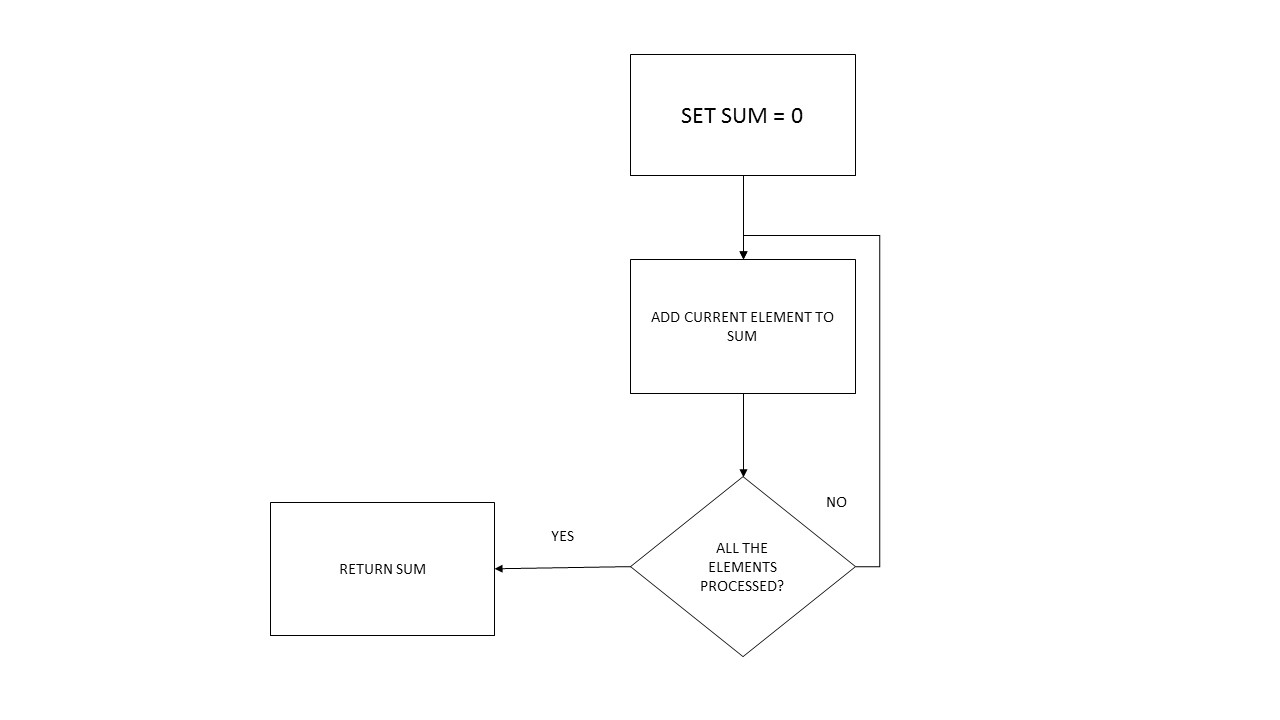
\includegraphics[width = \textwidth]{Figures/flow_chart}
	\caption{Flow chart for the sum of a sequence of numbers}
	\label{fig:ch1_flow_chart}
\end{figure}

\subsubsection*{Pseudocode}
Pseudocode is a semi-formal language that might contain also statements expressed in natural language and omits system specific code like opening file writers, printing messages on the standard output, or even some data structure declaration and initialization. It is intended mainly for human reading rather than machine reading. The pseudocode to sum a sequence of numbers is shown in Algorithm \ref{alg:ch1_pseudocode}.

\begin{algorithm}
	\caption{Pseudocode to perform the sum of a sequence of integer numbers}
	\label{alg:ch1_pseudocode}
	\begin{algorithmic}
		\Function{SumIntegers}{$l \text{ list of integers}$}
			\State $sum \gets 0$
			\ForAll {$x \text{ in } l$}
				\State $sum \gets sum + x$
			\EndFor
			\State \Return $sum$
		\EndFunction
	\end{algorithmic}
\end{algorithm}

\subsubsection*{Advantages and disadvantages}
Using flow charts or pseudo-code has the advantage of being able to define an algorithm in a way which is very close to the abstractions employed when using natural language: a flow chart combines both the use of natural language and a visual interface to describe an algorithm, pseudo-code allows to employ several abstractions and even define some steps in terms of natural language. The drawback of these two formal representations is that, when it comes to the implementation, the definition of the algorithm must be translated by hand into code that the hardware is able to execute. This could be done by implementing the algorithm in a low-level or high-level programming language. This process affects at different levels how the logic of the algorithm is presented, as explained further.

\section{Programming languages}
\label{sec:ch1_programming_languages}
A programming language is a formal language that is used to define instructions that a machine, usually a computer, must perform in order to produce a result through computation \cite{mordechai1996, narasimhan1967programming, oxford2008}. There is a wide taxonomy used to classify programming languages depending on their use \cite{kelleher2005lowering, myers1986visual, myers1990taxonomies}, but all can be grouped according to two main characteristics: the level of abstraction, or how close to the specific targeted hardware they are, and the domain, which defines the range of applicability of a programming language. In the following sections we give an exhaustive explanation of the aforementioned characteristics.

\subsection{Low-level programming languages}
\label{subsec:ch1_ll_languages}
A low-level programming language is a programming language that provides little to no abstraction from the hardware architecture of a processor. This means that it is strongly connected with the instruction set of the targeted machine, the set of instructions a processor is able to execute. These languages are divided into two sub-categories: \textit{first-generation} and \textit{second-generation} languages:

\subsubsection*{First-generation languages}
\textit{Machine code} falls into the category of first-generation languages. In this category we find all those languages that do not require code transformations to be executed by the processor. These languages were used mainly during the dawn of computer age and are rarely employed by programmers nowadays. Machine code is made of stream of binary data, that represents the instruction codes and their arguments \cite{guide2011intel, seal2001arm}. Usually this stream of data is treated by programmers in hexadecimal format, which is then remapped into binary code. The programs written in machine code were once loaded into the processor through a front panel, a controller that allowed the display and alteration of the registers and memory (see Figure \ref{fig:ch1_front_panel}). An example of machine code for a program that computes the sum of a sequence of integer numbers can be seen in Listing \ref{lst:ch1_machine_code}.

\begin{figure}
	\centering
	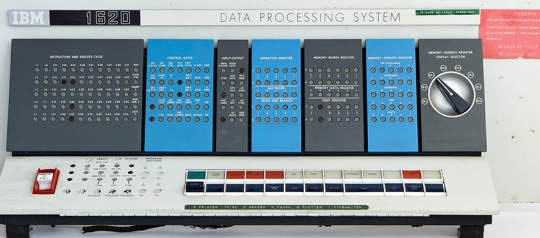
\includegraphics[width = \textwidth]{Figures/ch1_front_panel}
	\caption{Front panel of IBM 1620}
	\label{fig:ch1_front_panel}
\end{figure}

\begin{minipage}{\linewidth}
\begin{lstlisting}[numbers = left, caption = Machine code to compute the sum of a sequence of numbers, label = lst:ch1_machine_code]
 00075	c7 45 b8 00 00
 00 00
 0007c	eb 09	
 0007e	8b 45 b8
 00081	83 c0 01
 00084	89 45 b8
 00087	83 7d b8 0a
 0008b	7d 0f
 0008d	8b 45 b8
 00090	8b 4d c4
 00093	03 4c 85 d0
 00097	89 4d c4
 0009a	eb e2
\end{lstlisting}
\end{minipage}

\subsubsection*{Second-generation languages}
The languages in this category provides an abstraction layer over the machine code by expressing processor instructions with mnemonic names both for the instruction code and the arguments. For example, the arithmetic sum instruction \texttt{add} is the mnemonic name for the instruction code \texttt{0x00} in \texttt{x86} processors. Among these languages we find \textit{Assembly}, that is mapped with an \textit{Assembler} to machine code. The Assembler can load directly the code or link different \textit{object files} to generate a single executable by using a \textit{linker}. An example of assembly \texttt{x86} code corresponding to the machine code in Listing \ref{lst:ch1_machine_code} can be found in Listing \ref{lst:ch1_assembly_code}. You can see that the code in the machine code \texttt{00081	83 c0 01} at line 5 has been replaced by its mnemonic representation in Assembly as \texttt{add	eax, 1}.

\begin{minipage}{\linewidth}
\begin{lstlisting}[numbers = left, caption = Assembly x86 code to compute the sum of a sequence of numbers, label = lst:ch1_assembly_code]
mov	DWORD PTR _i$1[ebp], 0
jmp	SHORT $LN4@main
$LN2@main:
mov	eax, DWORD PTR _i$1[ebp]
add	eax, 1
mov	DWORD PTR _i$1[ebp], eax
$LN4@main:
cmp	DWORD PTR _i$1[ebp], 10			; 0000000aH
jge	SHORT $LN3@main
mov	eax, DWORD PTR _i$1[ebp]
mov	ecx, DWORD PTR _sum$[ebp]
add	ecx, DWORD PTR _numbers$[ebp+eax*4]
mov	DWORD PTR _sum$[ebp], ecx
jmp	SHORT $LN2@main
\end{lstlisting}
\end{minipage}

\subsubsection*{Advantages and disadvantages}
Writing a program in low-level programming languages might produce programs that are generally more efficient than their high-level counterparts, as ad-hoc optimizations are possible. However, the high-performance comes at great costs: (\textit{i}) the programmer must be an expert of the underlying architecture and of the specific instruction set of the processor, (\textit{ii}) the program loses portability because the low-level code is tightly bound to the specific hardware architecture it targets, (\textit{iii}) the logic and readability of the program is hidden among the details of the instruction set itself, and (\textit{iv}) developing a program in assembly requires a considerable effort in terms of time and debugging \cite{frampton2009demystifying}: assembly lacks any abstraction from the concrete hardware architecture, such as a type system, that partially ensures the correctness of the program or high-level constructs that allow to manipulate the execution of the program.

\subsection{High-level programming languages}
\label{subsec:ch1_hl_languages}
A high-level programming language is a programming language that offers a high level of abstraction from the specific hardware architecture of the machine. Unlike machine code (and in some way also assembly), high-level languages are not directly executable by the processor and they require some kind of translation process into machine code. The level of abstraction offered by the language defines how high level the language is. Several categories of high-level programming language exist, but the main one are described below.

\subsubsection*{Imperative programming languages}
\textit{Imperative programming languages} model the computation as a sequence of statements that alter the state of the program (usually the memory state). A program in such languages consists then of a sequence of \textit{commands}. Notable examples are FORTRAN, C, and PASCAL. An example of the program used in Listing \ref{lst:ch1_machine_code} and \ref{lst:ch1_assembly_code} written in C can be seen in Listing \ref{lst:ch1_c_code}. Line 5 to 9 corresponds to the Assembly code in Listing \ref{lst:ch1_assembly_code}.

\begin{lstlisting}[numbers = left, caption = C code to compute the sum of a sequence of numbers, label = lst:ch1_c_code]
int main()
{
  int numbers[10] = { 1, 6, 8, -2, 4, 3, 0, 1, 10, -5 };
  int sum = 0;
  for (int i = 0; i < 10; i++)
  {
    sum += numbers[i];
  }
  printf("%d\n", sum);
}
\end{lstlisting}

\subsection*{Declarative programming languages}
\textit{Declarative programming languages} are antithetical to those based on imperative programming, as they model computation as an evaluation of expressions and not as a sequence of commands to execute. Declarative programming languages are called as such when they are side-effects free or referentially transparent. The definition of referential transparency varies \cite{quine2013word}, but it is usually explained with the substitution principle, which states that a language is referentially transparent if any expression can be replaced by its value without altering the behaviour of the program \cite{mitchell2003concepts}. For instance, the following sentences in natural language are both true

\begin{lstlisting}
Cicero = Tullius

''Cicero`` contains six letters
\end{lstlisting} 

\noindent
but they are not referentially transparent, since replacing the last name with the middle name falsifies the second sentence.

A similar situation in programming languages is met when considering variable assignments: the statement

\begin{lstlisting}
x = x + 5
\end{lstlisting}

\noindent
is not referentially transparent. Let us assume this statement appears twice in a program and that at the beginning x = 0. Clearly the expression \texttt{x + 5} results in the value 5 the first time, but the second time the same statement is executed the expression has value 10. Thus replacing all the occurrences of \texttt{x + 5} with 5 is wrong, which is why imperative languages are not referentially transparent. A more rigorous definition of referential transparency can be found in \cite{sondergaard1990referential}.

Declarative programming languages are often compared to imperative programming languages by stating that declarative programming defines \textit{what} to compute and not \textit{how} to compute it. This family of languages include \textit{functional programming}, \textit{logic programming}, and \textit{database query languages}. Notable examples are F\#, Haskell, Prolog, SQL, and Linq (which is a query language embedded in C\#). Listing \ref{lst:ch1_fsharp_code_rec} shows the code to perform the sum of a sequence of integer numbers in F\# with a recursive function. Higher-order functions, such as \texttt{fold}, allow even to capture the same recursive pattern into a single function as shown in Listing \ref{lst:ch1_fsharp_code_fold}. Both implementations are referentially transparent.

\begin{lstlisting}[caption = Recursive F\# code to compute the sum of a sequence of numbers, label = lst:ch1_fsharp_code_rec]
let rec sumList l =
  match l with
  | [] -> 0
  | x :: xs -> x + (sumList xs)
\end{lstlisting}

\begin{lstlisting}[caption = F\# code to compute the sum of a sequence of numbers using higher-order functions, label = lst:ch1_fsharp_code_fold]
let sumList l = l |> List.fold (+) 0
\end{lstlisting}

\subsection{General-purpose vs Domain-specific languages}
\label{sec:ch1_dsl}
\textit{General-purpose languages} are defined as languages that can be used across different application domains and lack abstractions that specifically target elements of a single domain. Example of these are languages such as C, C++, C\#, and Java. Although several applications are still being developed by using general-purpose programming languages, in several contexts it is more convenient to rely on \textit{domain-specific languages}, because they offer abstractions relative to the problem domain that are unavailable in general-purpose languages \cite{van2000domain, voelter2013dsl}. Notable examples of the use of domain-specific languages are listed below.

\subsubsection*{Graphics programming}
Rendering a scene in a 3D space is often performed by relying on dedicated hardware. Modern graphics processors rely on shaders to create various effects that are rendered in the 3D scene. Shaders are written in domain-specific languages, such as GLSL or HLSL \cite{glhl2014, hlsl2018, hlslref2018}, that offer abstractions to compute operations at GPU level that are often used in computer graphics, such as vertices and pixel transformations, matrix multiplications, and interpolation of textures. Listing \ref{lst:ch1_hlsl_code} shows the code to implement light reflections in HLSL. At line 4 you can, for example, see the use of matrix multiplication provided as a language abstraction in HLSL.

\begin{lstlisting}[numbers = left, caption = HLSL code to compute the light reflection, label = lst:ch1_hlsl_code]
VertexShaderOutput VertexShaderSpecularFunction(VertexShaderInput input, float3 Normal : NORMAL)
{
  VertexShaderOutput output;
  float4 worldPosition = mul(input.Position, World);
  float4 viewPosition = mul(worldPosition, View);
  output.Position = mul(viewPosition, Projection);
  float3 normal = normalize(mul(Normal, World));
  output.Normal = normal;
  output.View = normalize(float4(EyePosition,1.0f) - worldPosition);
  return output;
}
\end{lstlisting}

\subsubsection*{Game programming}
Computer games are a field where domain-specific languages are widely employed, as they contain complex behaviours that often require special constructs to model timing event-based primitives, or to execute tasks in parallel. These behaviours cannot be modelled, for performance reasons, by using threads. Therefore, in the past, domain-specific languages which provide these abstractions have been implemented \cite{nwnlexicon2018, jass2011, unrealscript2018, sqf2018}. In Listing \ref{lst:ch1_sqf_code} an example of the SQF domain-specific language for the game ArmA2 is shown. This language offers abstractions to wait for a specific amount of time, to wait for a condition, and to spawn scripts that run in parallel to the callee, that you can respectively see at lines 18, 12, and 10.

\begin{lstlisting}[numbers = left, caption = ArmA 2 scripting language, label = lst:ch1_sqf_code]
"colorCorrections" ppEffectAdjust [1, pi, 0, [0.0, 0.0, 0.0, 0.0], [0.05, 0.18, 0.45, 0.5], [0.5, 0.5, 0.5, 0.0]];  
"colorCorrections" ppEffectCommit 0;  
"colorCorrections" ppEffectEnable true;

thanatos switchMove "AmovPpneMstpSrasWrflDnon";
[[],(position tower) nearestObject 6540,[["USMC_Soldier",west]],4,true,[]] execVM "patrolBuilding.sqf";
playMusic "Intro";

titleCut ["", "BLACK FADED", 999];
[] Spawn 
{
	waitUntil{!(isNil "BIS_fnc_init")};
	[
	  localize "STR_TITLE_LOCATION" ,
	  localize "STR_TITLE_PERSON",
	  str(date select 1) + "." + str(date select 2) + "." + str(date select 0)
	] spawn BIS_fnc_infoText;
	sleep 3;
	"dynamicBlur" ppEffectEnable true;   
	"dynamicBlur" ppEffectAdjust [6];   
	"dynamicBlur" ppEffectCommit 0;     
	"dynamicBlur" ppEffectAdjust [0.0];  
	"dynamicBlur" ppEffectCommit 7;
	titleCut ["", "BLACK IN", 5];
};
\end{lstlisting}

\subsubsection*{Shell scripting languages}
Shell scripting languages, such as the \textit{Unix Shell script}, are used to manipulate files or user input in different ways. They generally offer abstractions to the operating system interface in the form of dedicated commands. Listing \ref{lst:ch1_shell_code} shows an example of a program written in Unix shell script to convert an image from JPG to PNG format. At line 3 you can see the use of the statement \texttt{echo} to display a message in the standard output.

\begin{lstlisting}[numbers = left, caption = Unix shell code, label = lst:ch1_shell_code]
for jpg; do                                  
  png="${jpg%.jpg}.png"                    
  echo converting "$jpg" ...               
  if convert "$jpg" jpg.to.png ; then      
    mv jpg.to.png "$png"                 
  else                                     
    echo 'jpg2png: error: failed output saved in "jpg.to.png".' >&2
    exit 1
  fi                                       
done                                         
echo all conversions successful              
exit 0
\end{lstlisting}

\subsubsection*{Advantages and disadvantages}
High-level programming languages offer a variety of abstractions over the specific hardware the program targets. The obvious advantage of this is that the programmer does not need to be an expert of the underlying hardware architecture or instruction set. A further advantage is that the available abstractions are closer to the semi-formal description of the underlying algorithm as pseudo-code. This produces two desirable effects: (\textit{i}) the readability of the program is increased as the available abstractions are closer to the natural language than the equivalent machine code, and (\textit{ii}) that being able to mimic the semi-formal version of an algorithm, which is generally how the algorithm is presented and on which its correctness is proven, grants a higher degree of correctness in the specific implementation.

The use of a high-level programming language might, in general, not achieve the same high-performance as writing the same program with a low-level programming language  \cite{chatzigeorgiou2002evaluating}, but modern code-generation optimization techniques can generally mitigate this gap \cite{amarasinghe1993communication, wang2007code}. A further major issue in using high-level programming languages is that the machine cannot directly execute the code, thus the use of a compiler that translates the high-level program into machine code is necessary.

The portability of a high-level programming language depends on the architecture of the underlying compiler, thus some languages are portable and the same code can be run on different machines (for example Java), while others might require to be compiled to target a specific architecture (for example C++).

\section{Compilers}
\label{sec:ch1_compilers}
A compiler is a program that transforms source code defined in a programming language into another computer language, which usually is object code but can also be code in a high-level programming language \cite{aho2007compilers, appel2002javacompiler}. Writing a compiler is a necessary step to implementing a high-level programming language. Indeed, a high-level programming language, unlike low-level ones, are not executable directly by the processor and need to be translated into machine code, as stated in Section \ref{subsec:ch1_ll_languages} and \ref{subsec:ch1_hl_languages}.

The first complete compiler was developed by IBM for the FORTRAN language and required 18 person-years for its development \cite{backus1957fortran}. This clearly shows that writing a compiler is a hard and time-consuming task.

A compiler is a complex piece of software made of several components that implement a step in the translation process. The translation process performed by a compiler involves the following steps:

\begin{enumerate}
	\item \textit{syntactical analysis:} In this phase the compiler checks that the program is written according to the grammar rules of the language. In this phase the compiler must be able to recognize the \textit{syntagms} of the language (the ``words'') and also check if the program conforms to the syntax rules of the language through a grammar specification.
	\item \textit{type checking:} In this phase the compiler checks that a \textit{syntactically correct program} performs operations conform to a defined \textit{type system}. A type system is a set of rules that assign properties called types to the constructs of a computer program \cite{pierce2002types}. The use of a type system drastically reduces the chance of having bugs in a computer program \cite{cardelli1996type} . This phase can be performed at compile time (\textit{static typing}) or the generated code could contain the code to perform the type checking at runtime (\textit{dynamic typing}). 
	\item \textit{code generation:} In this phase the compiler takes the \textit{syntactically and type-correct program} and performs the translation step. At this point an equivalent program in a target language will be generated. The target language can be object code, another high-level programming language, or even a bytecode that can be interpreted by a virtual machine.
\end{enumerate}

All the previous steps are always the same regardless of the language the compiler translates from and they are not part of the creative aspect of the language design \cite{book1970cwic}. Approaches to automating the construction of the syntactical analyser are well known in literature \cite{mcpeak2004elkhound, nivre2006maltparser, parr1995antlr}, to the point that several lexer/parser generators are available for programmers, for example all those belonging to the \texttt{yacc} family such as \texttt{yacc} for C/C++, \texttt{fsyacc} for F\#, \texttt{cup} for Java, and \texttt{Happy} for Haskell. On the other hand, developers lack a set of tools to automate the implementation of the last two steps, namely the type checking and the code generation.

For this reason, when implementing a compiler, the formal type system definition and the operational semantics, which is tightly connected to the code generation and defines how the constructs of the language behave, must be translated into the abstractions provided by the host language in which the compiler will be implemented. Other than being a time-consuming activity itself, this causes that (\textit{i}) the logic of the type system and operational semantics is lost inside the abstraction of the host-language, and (\textit{ii}) it is difficult to extend the language with new features.

\section{Meta-compilers}
\label{sec:ch1_metacompilers}
In Section \ref{sec:ch1_compilers} we described how the steps involved in designing and implementing a compiler do not require creativity and are always the same, regardless of the language the compiler is built for. The first step, namely the syntactical analysis, can be automated by using one of the several lexer/parser generators available, but the implementation of a type checker and a code generator still relies on a manual implementation. This is where meta-compilers come into play: a meta-compiler is a program that takes the source code of another program written in a specific language and the language definition itself, and generates executable code. The language definition is written in a programming language, referred to as \textit{meta-language}, which should provide the abstractions necessary to define the syntax, type system, and operational semantics of the language, in order to implement all the steps above.

\subsection{Requirements}
As stated in Section \ref{sec:ch1_metacompilers}, a meta-compiler should provide a meta-language that is able to define the syntax, type system, and operational semantics of a programming language. In Section \ref{sec:ch1_compilers} we discussed how methods to automate the implementation of syntactical analyser are already known in scientific literature. For this reason, in this work, we will focus exclusively on automating the implementation of the type system and of the operational semantics. Given this focus, we formulate the following requirements:

\begin{itemize}
	\item The meta-language should provide abstractions to define the constructs of the language. This includes the possibility of defining control structures, operators with any form of prefix or infix notation, and the priority of the constructs that is used when evaluating their behaviour. Furthermore, it must be possible to define the equivalence of language constructs. For instance, an integer constant might be considered both a value and a basic arithmetic expression.
	
	\item The meta-language must be able to mimic as close as possible the formal definition of a programming language. This will bring the following benefits: (\textit{i}) Implementing the language in the meta-compiler will just involve re-writing almost one-to-one the type system or the semantics of the language with little or no change; (\textit{ii}) the correctness and soundness \cite{cardelli1996type, milner1972proving} of the language formal definition will be directly reflected in the implementation of the language; indeed if a meta-program allows to mimic directly the type system and semantics of the language their correctness is transferred also in the implementation, while this might not be trivial when translating them in the abstractions of a high-level programming language; (\textit{iii}) any extension of the language definition can be just added as an additional rule in the type system or the semantics.
	
	\item The meta-compiler must be able to embed libraries from external languages, so that they can be used to implement specific behaviours such as networking transmission or specific data structure usage.
\end{itemize}

\subsection{Benefits}
\label{sec:ch1_benefits}
%list the benefits first and then explain. Add a paragraph also about correctness
Programming languages usually are released with a minimal (but sufficient to be Turing-complete) set of features, and later extended in functionality in successive versions. This process tends to be slow and often significant improvements or additions are only seen years after the first release. For example, Java was released in 1996 and lacked an important feature such as Generics until 2004, when J2SE 5.0 was released. Furthermore, Java and C++ lacked constructs from functional programming, which is becoming more and more popular with the years \cite{thompson1995miranda}, such as lambda abstractions until 2016, while a similar language like C\# 3.0 was released with such capability in 2008. The slow rate of change of programming languages is due to the fact that every abstraction added to the language must be reflected in all the modules of its compiler: the grammar must be extended to support new syntactical rules, the type checking of the new constructs must be added, and the appropriate code generation must be implemented. Given the complexity of compilers, this process requires a huge amount of work, and it is often obstructed by the low flexiblity of the compiler as piece of software. Using a meta-compiler would speed up the extension of an existing language because it would require only to change on paper the type system and the operational semantics, and then add the new definitions to their counterpart written in the meta-language. This process is easier because the meta-language should mimic as close as possible their behaviour. Moreover, backward compatibility is automatically granted because an older program will simply use the extended language version to be compiled by the meta-compiler.

To this we add the fact that, in general, for the same reasons, the development of a new programming language is generally faster when using a meta-compiler. This could be beneficial to the development of a high variety of domain-specific languages. Indeed, such languages are often employed in situations where the developers have little or no resources to develop a fully-fledged hard-coded compiler by hand. For instance, it is desirable for game developers to focus on aspects that are strictly tied to the game itself, for example the development of an efficient graphics engine or to improve the game logic. At the same time they would need a domain-specific language to express some behaviours typical of games, things that could be achieved by using a meta-compiler rather than on a hand-made implementation.

\subsection{Scientific relevance} %change the tile
\label{sec:ch1_scientific_relevance}
Meta-compilers have been researched since the 1960's \cite{schorre1964meta} and several implementations have been proposed \cite{ braborovansky1998overview, venboer2008stratego, klint2009rascal, pettersson1996compiler, verdejo2006executable}. In general meta-compilers perform poorly compared to hard-coded compilers because they add the additional layer of abstraction of the meta-language. Moreover, a specific implementation of a compiler opens up the possibility of implementing language-specific optimizations during the code generation phase. Meta-compilers have been used in a wide range of applications, such as source code analysis and manipulation and physical simulations \cite{kaagedal1998generating}, but no use up to our knowledge was made in the field of domain-specific languages for games. Since games are pieces of software that are very demanding in terms of performance, we think that it could be of interest to investigate the applicability of meta-compilers in the scope of domain-specific languages for games and the development speed up introduced by the use of such a tool. In this work we present Metacasanova, a meta-compiler based on natural semantics that was born from the intent of easing the development of the domain-specific language for game development Casanova, and we analyse the benefit of using it for a re-implementation and extension of Casanova.

\section{Problem statement}
\label{sec:ch1_problem_statement}
In Section \ref{sec:ch1_programming_languages} we showed the advantages of using high-level programming languages when implementing an algorithm. Among such languages, it is sometimes desirable to employ domain-specific languages that offer abstractions relative to a specific application domain (Section \ref{sec:ch1_dsl}). In Section \ref{sec:ch1_compilers} we described the need of a compiler for such languages, and that developing one is a time-consuming activity despite the process being, in great part, non-creative. In Section \ref{sec:ch1_metacompilers} we introduced the role of meta-compilers to speed up the process of developing a compiler and we listed the requirements and the benefits that one should have. In Section \ref{sec:ch1_scientific_relevance} we explained why we believe that meta-compilers are a relevant scientific topic if coupled with the problem of of developing domain-specific languages in response to the their increasing need. We can now formulate our problem statement:

\vspace{0.5cm}
\noindent
\textbf{Problem statement: } \textit{\psContent}

\vspace{0.5cm}
\noindent
The first parameter we need to evaluate in order to answer this question is the size of the code reduction needed to implement the domain-specific language. At this purpose, the following research question arises:

\vspace{0.5cm}
\noindent
\textbf{Research question 1: } \textit{\rqContentOne}

\vspace{0.5cm}
\noindent
The second parameter we need to evaluate is the eventual performance loss caused by introducing the abstraction layer provided by the meta-compiler. This leads to the following research question:

\vspace{0.5cm}
\noindent
\textbf{Research question 2: } \textit{\rqContentTwo}

\vspace{0.5cm}
\noindent
In case of a performance loss, we need to identify the cause of this performance loss and if an improvement is possible. This leads to the following research question:

\vspace{0.5cm}
\noindent
\textbf{Research question 3: } \textit{\rqContentThree}

\vspace{0.5cm}
\noindent

\section{Thesis structure}
This thesis describes the architecture of Metacasanova, a meta-compiler whose meta-language is based on operational semantics, and a possible optimization for such meta-compiler. It also shows its the capabilities by implementing a small imperative language and re-implementing the existing domain-specific language for games \textit{Casanova 2}, extending it with abstractions to express network operations for multiplayer games.

In Chapter \ref{ch:background} we provide background information in order to understand the choices made for this work. The chapter presents the state of the art in designing and implementing compilers and existing research on meta-compilers.

In Chapter \ref{ch:metacasanova} we present the architecture of Metacasanova by extensively describing the implementation of all its modules.

In Chapter \ref{ch:languages} we show how to use Metacasanova to implement two languages: a small imperative language, and \textit{Casanova 2}, a language for game development. At the end of the chapter we provide an evaluation of the performance of the two languages and their implementation length with respect to existing compilers, thus answering to Research Question 1 and 2.

In Chapter \ref{ch:functors} we discuss the performance loss of the implementation of the presented languages and we propose an extension of Metacasanova that aims to improve the performance of the generated code, thus answering Research Question 3.

In Chapter \ref{ch:functor_languages} we show how to use functors to improve the performance of Casanova implemented in Metacasanova, comparing this approach and the one presented in Chapter \ref{ch:languages} with respect to the execution time of a sample in Casanova. 

In Chapter \ref{ch:networking} we propose an extension of Casanova 2 for multiplayer game development. We first provide its hard-coded compiler solution and then we show how to extend the implementation in the meta-compiler to include the same extension. In this chapter we evaluate the performance of a multiplayer game implemented in Casanova with this extension with respect to the same game implemented in C\#, and we measure the effort of realising such extension in the hard-coded compiler of Casanova versus the implementation with Metacasanova.

In Chapter \ref{ch:discussion} we discuss the result and answer the research questions.

\section{PROBLEM - An analysis of RTS's}
Within the context of higher education, learning programming is hard for both beginners and students with past experience. 

It is suggested by some \cite{tan2009learning} that learning programming is no different than most other complex skills: it takes roughly ten years (ten thousand hours) to become truly proficient.

The reason why it takes so long is disarmingly simple. Programming requires both the ability to \textit{understand} and to \textit{design} code. 

\subsection{Understanding code}
Understanding code is a passive skill, but not any simpler because of it. The true meaning of code is the sequence of steps that the machine will actually perform: every single bit that will be read and written as a result of an instruction is part of the meaning of that instruction, just like every cache hit-or-miss, the activation of the CPU ALU(s), network channels, operating systems, interpreters, just-in-time compilers, and ultimately interactions with users. Being able to figure precisely what a program does, and how it does it (also in terms of performance) requires the ability to formulate an abstract idea of the program behaviour, and the mapping of this \textit{abstract idea} to the concrete components when more specific reasoning is needed.

The sheer size of the machinery involved in the execution of even the simplest program is simply \textit{very large}, and \textit{the ability to think hierarchically and zoom in and out of the details as needed takes a lot of experience}.

\subsection{Designing code}
Designing code is an active skill, and as such intrinsically complex. Designing code requires the formulation (and therefore the choice) of a design strategy, usually in a top-down fashion, which is then recursively turned into a more and more concrete definition of the program. Being able to design a program effectively requires the ability to choose a specific design among a series of possible designs, which taken together form \textit{the abstract meta-strategies} that characterise a programmer’s knowledge, style, and experience.

The sheer size of the design space of even the simples program is \textit{so large as to be essentially infinite} (we are talking about finite machines after all!), and the ability to \textit{formulate meta-strategies and employ them recursively takes a lot of experience}.

\subsection{Size matters (and so does structure)}
We believe the size of the domain to be the core of the issue. Even though some students might already know a few tricks to produce working programs in some very narrow domain, the fundamental ability to abstractly reason about code (both for understanding and designing programs) is usually severely lacking in first year students.

Moreover, we cannot just solve the problem by throwing unstructured assignments such as “read this code” or “try and write this program”, as we must train the specific mental activities that we wish to stimulate in students. Specific training must be structured in order to gently guide the activation of the proper thought structures, in a slow buildup of complexity and freedom to express one’s own creativity.

\subsection{The issues}
We close this session by identifying a series of practical, concrete issues that we believe sum up the discussion so far:

\begin{table}[!h]
	\begin{tabular}{|c|p{8cm}|}
		\hline
		\textbf{ID} & \textbf{Issue} \\
		\hline
		REASON\textunderscore MODEL & Students need extensive practice with reasoning about models of programs \\
		\hline
		REASON\textunderscore DESIGN & Students need extensive practice with reasoning about existing design strategies \\
		\hline
		EXTEND\textunderscore DESIGN & Students need extensive practice with extending existing programs (which should follow a formative design). \\
		\hline
		EXTEND\textunderscore BUILDUP & Students need a buildup in complexity with their extension activities. \\
		\hline
	\end{tabular}
	\caption{Issues about learning programming}
	\label{tab:issues}
\end{table}

By keeping these issues in mind, we will now setup a proposed didactic model which we believe can mitigate them or outright resolve them.






\section{``Galaxy Wars" case study}
Mini Galaxy Wars.



\section{SOLUTION - Our idea}
Casanova 2 is an iteration of Casanova, a DSL for game development. A Casanova program is a tree of data structures called \textit{entities}. The root of the tree is called \textit{world}. Each entity contains a set of \textit{rules} which modifies the fields and describe continuous dynamics. Discrete dynamics (the dynamics of the game that require timing or synchronization conditions) are expressed by coroutines implemented with a variation of the state monad. Casanova 2 eliminates this separation by allowing rule to be interruptible, thus describing both continuous and discrete dynamics. The rule body is looped continuously, which means that once the evaluation reaches the end, the rule is re-started from the first statement. Writing entity fields is allowed only by using rules. A rule can write an entity field by using a dedicated \texttt{yield} statement. Each rule declares a subset of fields called \textit{domain} on which it is allowed to write. Besides each rule has an implicit reference to the world (variable \texttt{world}), the current entity (variable \texttt{this}), and the time difference between the current frame and the previous (variable \texttt{dt}). Casanova 2 supports interruptible control structures and queries, so it natively supports REA.

\section{REACDM Galaxy Wars in Casanova 2}
We now show that Casanova 2 is able to express the design of Galaxy Wars in terms of REA. In what follows the type $[T]$ denotes a list of objects of type $T$, according to Casanova 2 syntax. We begin by defining the structure of the world entity. The world contains the collection of \texttt{Planets} in the map, the collection of \texttt{Links} connecting the planets, the collection of \texttt{Players}, and a \texttt{Controller} that manages the input controller and provides facilities like: the current selected planet, whether a mouse button is down, etc.

\begin{lstlisting}
worldEntity GalaxyWars =
  Planets    : [Planet]
  Links      : [Link]
  Players    : [Player]
  Controller : Controller 
  
  //rules
\end{lstlisting}



\subsection{Resources}
The resources are all those elements that influence the game dynamics. In Galaxy Wars the resources are: 


\begin{itemize}[noitemsep]
\item amount of fleets in a Planet
\item the player statistics (attack, defence, production, research)
\item planet and the ships statistics
\item the amount of travelling ships in a link
\end{itemize}

\noindent
We use the following properties to model the statistics of the entities: player, planet, and fleet.

\begin{lstlisting}
entity GameStatistics =
  Attack               : float32
  Defence              : float32
  Production           : float32
  Research             : float32
\end{lstlisting}



\subsection{Entities}
Entities represent the resource containers in Galaxy Wars. The entities in Galaxy Wars are: \texttt{Planets}, \texttt{Fleets}, \texttt{Players}, and \texttt{Links}. A player represents the commander managing all the elements of the RTS. It contains starting statistics that define a faction (a player might start with more production but less research). During the game statistics can be increased with upgrades.

\begin{lstlisting}
entity Player =
  Statistics          : GameStatistics
  Name                : string
\end{lstlisting}

\noindent
A planet represents the container of stationed ships. Each planet has its own statistics. The attack capabilities of a fleet can be increased depending on the attack value of the source planet. Research affects the velocity of the outgoing fleet. Defense and production affects the ship construction speed and defence capabilities (used when a planet is attacked). We use inbound fleets to select the incoming fleets from a link that is targeting the current planet. \texttt{Owner} is an option because not all planets are controlled by a player (in the beginning every player owns at most one planet and the other are neutral).

\begin{lstlisting}
entity Planet =
  Statistics          : GameStatistics
  LocalFleets         : int
  InboundFleets       : [Fleet]
  ref Owner           : Option<Player>
  Battle              : Option<Battle>
  
  
  //rules
\end{lstlisting}

\noindent
A \texttt{Fleet} is defined by an \texttt{Owner}, the amount of ships, and its own statistics. Attack and defence are used in combat. A fleet has no production (it is always set to 0), while the research defines its speed.

\begin{lstlisting}
entity Fleet =
  Statistics          : GameStatistics
  Ships               : int
  ref Owner           : Player
  
  //rules
\end{lstlisting}


\noindent
Battles in GalaxyWars are carried out by mean of entities of type \texttt{Battle}. A battle is made up by:
\begin{itemize}
	\item \texttt{MySource} the planet where the battle is hosted, 	
	\item \texttt{AttackingFleets} the fleets that are waiting to attack \texttt{MySource},
	\item \texttt{SelectedAttackingFleet} the fleet that is attacking \texttt{MySource},
	\item \texttt{DefenceLost} the amount of fleets lost after a match by \texttt{MySource}, and
	\item \texttt{AttackLost} the amount of fleets lost after a match by \texttt{SelectedAttackingFleet}.
\end{itemize}

\begin{lstlisting}
entity Battle =
  ref MySource    : Planet
  AttackingFleets : [AttackingFleet] 
  SelectedAttackingFleet : Option<AttackingFleets>
  DefenceLost   : Option<int>
  AttackLost    : Option<int>
  
  //rules  
\end{lstlisting}

\noindent
A link is a directed connection between two planets. Besides its \texttt{Source} and \texttt{Destination}, a link also contains \texttt{TravellingFleets} that is collection of ships that are currently traveling along the link. 

\begin{lstlisting}
entity Link =
  ref Source             : Planet
  ref Destination        : Planet
  TravellingFleets   : [TravelingFleet]
  
  //rules
\end{lstlisting}

Eventually, we introduce two entities \texttt{TravelingFleet} and \texttt{AttackingFleet}. The former represent a fleet that is able to move around the map; the latter represents a ship able to carry out fighting tasks. A traveling fleet and an attacking fleet inherit the same \texttt{Fleet} entity. The reason is because an attacking ship is a traveling ship (same model, same position, same amount of fleets, etc.) that implements different set of behaviors. Furthermore, an attacking fleet contains also a reference its battle.

\begin{lstlisting}
entity AttackingFleet =
  inherit Fleet
  ref MyBattle : Battle
  //rules
  
entity TravelingFleet =
  inherit Fleet
  ref Destination : Planet
  //rules
\end{lstlisting}

\subsection{Actions}
Actions are the only way, according to REA, to exchange resources like the amount of attacks in a battle, the amount of fleets to produce, etc. In Galaxy Wars we identified three kind of actions: battle, production, and upgrade. Input actions are left out of our explanation, because the transfer behavior is not completely under the control of Casanova (input rely on external facilities/libraries). However, capturing user input in Casanova 2 is possible; some examples can be found on \url{https://github.com/vs-team/casanova-mk2/wiki/Casanova-Samples-and-Demos-Tutorials}. 
\\\\
\noindent
A \textbf{Battle} action involves a planet \texttt{MySource} and a series of \texttt{AttackingFleets}. In the following code The rule carries the attacking fleet selection. Every random time an entity among \texttt{AttackingFleets} is selected and stored into \texttt{SelectedAttackingFleet}. If in the mean time the battles ends we stop the selection and wait the battle to get disposed. If the selected ship is destroyed and there are \texttt{AttakingShips} available then we select an other attacking fleet among the \texttt{AttakingShips}.

\begin{lstlisting}
entity Battle =
  //fields
  
  rule SelectedAttackingFleet, AttackingFleets =
    .| SelectedAttackingFleet.Fleet.Destroyed && AttackingFleets = [] ->
       yield None, []
    .| SelectedAttackingFleet.Fleet.Destroyed ->
       let new_selected_fleet = AttackingFleets.[random(0, AttackingFleets.Count - 1)]
       yield new_selected_fleet, new_attacking_fleets - new_selected_fleet
    .| _ -> 
       wait random
       let new_selected_fleet = AttackingFleets.[random(0, AttackingFleets.Count - 1)]
       yield new_selected_fleet, new_attacking_fleets + SelectedAttackingFleet
  ...
\end{lstlisting}

\noindent
An other rule computes the amount of damage to apply every random amount of time to both \texttt{SelectedAttackingFleet} and \texttt{MySource}. 
\begin{lstlisting}
  ...
  rule DefenceLost, AttackLost =
    yield None, None
    wait random
    //code that computes the damage to apply to both
    //the attacker and defender based on their attack/defence
    //stats and on the mount of attacking fleets
\end{lstlisting}

\noindent
Every instance of \texttt{AttackingFleet} and \texttt{Planet} involved in a battle keep updating their amount of fleets, so to carry our their internal logic.
\begin{lstlisting}
entity AttackingFleet =
  //fields
  
  rule Destroyed =  wait Ships = 0; yield True
  rule Ships =
    wait MyBattle.AttackLost.IsSome && MyBattle.SelectedAttackingFleet = this
    yield Ships - MyBattle.AttackLost.Value
     
entity Planet =
  //fields and rules
  
  rule LocalFleets = 
    wait Battle.DefenceLost.IsSome
    yield LocalFleets - Battle.DefenceLost.Value
\end{lstlisting}

\noindent
We change the owner of a planet only in two possible ways: (\textit{i}) after the end of a battle and the attacker still got some armies alive, first rule (we set the current owner to \texttt{None}, after the victory of an attacking fleet, in order to reset the internal logics of the planet associated to the previous owner), and (\textit{ii}) when the planet is neutral and there are fleets that are inbounding, second rule. In the last case case the first fleet in \texttt{InboundFleets} gets the ownership.

\begin{lstlisting}
entity Planet =
  //fields and rules
  
  rule Owner = 
    wait Battle.IsSome && LocalFleets = 0 && 
    Battle.SelectedAttackingFleet.IsSome &&
    Battle.SelectedAttackingFleet.Value.Ships > 0
    yield None
    yield SelectedAttackingFleet.Value
    
  rule Owner, InboundFleets, LocalFleets = 
    wait Owner.IsNone && Battle.IsNone &&
         InboundFleets.Count > 0
    let selected_fleet = InboundFleets.Head
    yield selected_fleet.Owner,
          InboundFleets - selected_fleet 
          selected_fleet.Fleets
\end{lstlisting}

\noindent
A \textbf{production} action involves a \texttt{Planet} entity and the owner production statistics. The action is performed by a rule that waits an amount of time, which depends on the production statistics of both planet and owner, and then it adds a fleet to \texttt{LocalFleets}. If the planet changes owner (for a frame \texttt{Owner} is \texttt{None}) we reset the rule behavior and set \texttt{LocalFleets} to \texttt{0}.
\begin{lstlisting}
entity Planet =
  //other field and rules

  rules LocalFleets =
    .| Owner.IsNone -> yield 0
    .| _ ->
      wait Statistics.Production * Owner.Value.Production
      yield LocalFleets + 1
\end{lstlisting}

\textbf{Upgrading} the stats of a planet is performed by waiting the planet to get selected. When the planet is selected and a key associated to an upgrade is down we: (\textit{i}) wait an amount of time (which depends from the owner and the planet research statistics), then (\textit{ii}) we upgrade the selected statistic. If the planet is \texttt{Owner} less then its statistics are, by default, set to \texttt{1}.

\begin{lstlisting}
entity Planet = 
  //other field and rules

  rule Statistics.STAT =
    .| Owner.IsNone -> yield 1
    .| _ ->
      wait world.SelectedPlanet = this &&
           KeyPressed(STAT_KEY)
      wait Owner.Value.Research * Statistics.Research
      yield max(MAX_STAT, Statistics.STAT + 1)
\end{lstlisting}


\subsubsection{Creation}
In Galaxy Wars we create entities when: (\textit{i}) a battle is about to start, and (\textit{ii}) when a fleet is spawned.

\noindent
Given a planet \texttt{P}, a battle is created created if there are no other battles in progress in \texttt{P}, \texttt{P} is owned by a player, and \texttt{InboundFleets} contains at least an enemy fleet. A battle is disposed when the planet has lost its owner (\texttt{wait Owner.IsNone}) or when there are no \texttt{AttackingFleets} left.
\begin{lstlisting}
entity Planet =
  //fields and rules  

  rule Battle =
    wait Battle.IsNone && 
         Owner.IsSome &&
         InboundFleets.Contains(f => f.Owner <> Owner.Value)
    yield new Battle(this)
    wait Owner.IsNone
    yield None
\end{lstlisting}


\noindent
A fleet is sent though a link only if the source planet contains enough local fleets and there are no battles in progress. The local fleets of the selected planet are set to \texttt{0} when the user decides to send fleets through a link.

\begin{lstlisting}
entity Link =
  //fields and rules

  rule TravellingFleets, Source.LocalFleets = 
    wait world.SelectedPlanet = Source &&
         world.DestinationSelectedPlanet = Destination &&
         world.Battle.IsNone
         world.Source.LocalFleets > 0
    new TravelingFleet(new Fleet(Source, world.Source.LocalFleets)) @
        TravellingFleets, 0
\end{lstlisting}

\subsection{Deletion}
Analogously to creation, in GW the entities which might be disposed during a game are battles and fleets. 


The logic of the deletion of a battle is tightly related to the logic of its creation. In the code above a battle is disposed only when the \texttt{Owner} is \texttt{None}. This means that the planet owner has lost its owner, hence the battle is over.

The logic of the deletion of a fleet depends on whether the fleet is fighting or traveling. When fighting a fleet is destroyed when its life is below or equal to zero. When the life is below or equal to zero the fleet field \texttt{Destroyed} is set to \texttt{true}.
\begin{lstlisting}
entity AttackingFleet =
  inherit Fleet
  ref MyBattle : Battle
  rule Destroyed =
    wait Life <= 0.0f
    yield true
\end{lstlisting}

This is necessary in order to notify other entities that the fleet has been destroyed and to allow the battle to remove it from its \texttt{AttakingFleets}.
\begin{lstlisting}
entity Battle =  
  //fields and rules

  AttackingFleets : [Fleet]
  rule AttackingFleets =
    yield [for fleet in AttackingFleets do
           where not fleet.Destroyed
           select fleet]
\end{lstlisting}

When traveling, a fleet is destroyed upon it has reached its destination. In this case, when the fleet is among the \texttt{InboundFleets} of its \texttt{Destination} the field \texttt{Destroyed} of the fleet is set to \texttt{true}. An additional check is added before destroying the fleet. If the owner has changed or there is a battle running on the planet then the fleet should not be destroyed, since the fleet will turn into an attacking fleet. 
\begin{lstlisting}
entity TravelingFleet =
  inherit Fleet
  ref Destination : Planet
  rule Destroyed =
    wait self in Destination.InboundFleets &&
         Destination.Battle.IsNone         
    yield True
\end{lstlisting}

When a traveling fleet has reached its destination, the fleet is automatically filtered by the link. 
\begin{lstlisting}
entity Link =
  //fields
  rule TravellingFleets =
    yield [for f in TravellingFleets do
           where Vector3.Distance(f.Position, Destination.Position) > MIN_DIST
           select f]
\end{lstlisting}

\subsubsection{Change of strategy}
An entity during its life cycle might change its behavior based on its state. An example of this kind of behavior in GalaxWars could be identified with the fleet entity. For example an attacking fleets behaves differently than a moving fleet. In Casanova we distinguish these two cases by mean of two different entities that share some common properties, but implement different rules.

When a traveling fleet is approaching the planet at the end of the link, the planet has to choose whether to: (\textit{i}) add the fleet in the planet local fleets, (\textit{ii}) add the fleet to a battle, (\textit{iii}) or forward the fleet to an other link. To implement the just described scenario we start with the definition of a buffer to place in the \texttt{Planet} entity called \texttt{InboundFleets}. The \texttt{InboundFleets} of a planet \texttt{X} represents all fleets that are approaching at a specific moment the planet \texttt{X}. 

\begin{lstlisting}
entity Planet =  
  InboundFleets       : [Fleet]
  
  ..//other fields and rules
  
  rule InboundFleets =
    yield [for l in world.Links do           
           where l.Target = this &&
           for f in l.Fleets do
           where Vector3.Distance(f.Position, this.Position) < MIN_DIST
           select f.]

\end{lstlisting}

\texttt{InboundFleets} acts like a dispatcher. Entities are notified about change state of a fleet the moment it enters enters the \texttt{InboudFleets}. When a fleet enters the \texttt{InboundFleets} collection, other entities are able to consume it for their internal logics. To avoid entities to consume twice the same fleet, fleets in \texttt{InboundFleets} last for one frame before being disposed. When an entity consumes an inbound fleets it decides how to change the fleet behavior. 

\noindent
A battle entity every frame selects the enemy fleets from the inbound fleets of its \texttt{MySource} field and adds them to its \texttt{AttackingFleets}. Before adding the inbounding enemy fleets to the \texttt{AttackingFleets} collection, every inbound enemy fleet is converted to an attacking fleet.

\begin{lstlisting}
entity Battle =
  AttackingFleets : [AttackingFleet]
  rule AttackingFleets = 
    if MySource.Owner.IsSome then
      yield [for f in MySource.InboundFleets do
             where f.Owner <> MySource.Owner.Value
             select new AttackingFleet(f)] @ AttackingFleets
\end{lstlisting}

\noindent
A link forwards a fleet \texttt{F} to its own link when \texttt{F} is inside \texttt{Source.InboundFleets} and \texttt{F.NextTarget} is the link \texttt{Destination}.
\begin{lstlisting}
entity Link =
  ref Source             : Planet
  ref Destination        : Planet
  ref TravellingFleets   : [TravelingFleet]
  //... other rules
  rule TravelingFleets =
    wait Source.Battle.IsNone
    yield [for f in Source.InboundFleets do
           where f.NextTarget = Destination &&
           select new TravelingFleet(f)] @ TravellingFleets  
\end{lstlisting} 


\noindent
Eventually, a fleet is added to the local fleets of a planet if the fleet is in the \texttt{InboundFleets} collection and it shares the same owner of the planet.

\begin{lstlisting}
entity Planet = 
  LocalFleets   : int
  ref Owner     : Option<Player>
  InboundFleets : [InboundFleet]
  ...//other field and rules

  rules LocalFleets =
    wait Owner.IsSome
    yield LocalFleets + 
          [for f in InboundFleets do
           where Owner.Value = f.Owner
           select f
           sum]
\end{lstlisting}



\section{DETAILS - Abstraction}
In this section we show how Casanova 2 can implement the REA pattern, and also extend it with the CDM pattern.

\subsection{Resources}
Resources can be modeled as a Casanova entity with no rules containing a field for each of the resources used in the REA pattern. In a game we might have different resource entities for different group of resources. We define a resource entity by first defining its name \texttt{ResourceName} and then by listing the resources contained in it. A resource in Casanova is a field and it is defined as tuple \texttt{Resource * Type} where the first item refers to the field name while the latter refers to the field type. In the following we show a generalized description for a generic resource entity.

\begin{lstlisting}[mathescape]
entity ResourcesName =
  $\mathtt{R_{1} : T_{1}}$
  $\mathtt{R_{2} : T_{2}}$
  ...
  $\mathtt{R_{n} : T_{n}}$ 
\end{lstlisting}


\subsection{Entities}
REA entities can be modeled directly as Casanova entities. To avoid possible confusion arising from the ambiguity between the \texttt{entity} keyword in Casanova and entities in the REA pattern from now on we will refer to the latter as \textit{actors}. An actor will contain the \texttt{Resources} (of type ResourcesName) and a series of rules that will act as the constant, mutable, and threshold actions of REA.

\begin{lstlisting}
entity Actor = 
  Resources              : ResourcesName
  //constant actions
  //mutable actions
  //threshold actions
\end{lstlisting}

\subsection{Actions}
Following the REA pattern, we divide the actions into 3 categories: (\textit{i}) Constant transfer, (\textit{ii}) mutable transfer, and (\textit{iii}) threshold transfer. We model the REA transfers as rules in Casanova. 


An action in REA simply puts in communication a source with a target. In Casanova the source is the action/rule container while the target is an entity containing a field that refers to the source. Since very often actions are run only after a predicate is satisfied and the predicate might depends on the target properties, among the source fields a field that refers to the target is added. The target checks the source reference whenever it needs to interact with it. 

\noindent
A generalization for this approach could be the following: the source contains \texttt{S} a reference to a target \texttt{T}. Whenever the \texttt{T} needs to interact with an action it traverses the world to find an \texttt{S} that is targeting \texttt{T}. For practicality reasons from now on we use the not generalized version.


\noindent
The action rules do not modify the target actor directly to grant encapsulation, unless the target is the source itself. The source resources are read by the target actor periodically to locally update their fields\footnote{An extensive discussion about encapsulation in games, as well as an optimizer for encapsulated code in Casanova can be found in \cite{CASANOVA2_ENCAPSULATION}}. The resources to transfer generated by actions are stored inside the source entity and precisely inside its resource entity. We refer to the resources to transfer as \texttt{Transfers} in Casanova.

\noindent
The definition of the actions will be shown in the next three paragraphs.

\paragraph*{Constant transfer}
A constant transfer simply sums the resources of a source entity to the resources of the target. The following rule, which is contained in the source entity, updates the \texttt{Transfers} whenever a condition is met (we assume that \texttt{restrictions} is a predicate that specifies a condition to apply the action). The rule waits one frame, to ensure that the target actor reads the change, before resetting the \texttt{Transfers}.

\begin{lstlisting}[mathescape]
enity SourceActor =
  Resources   : ResourcesName
  ref TSource :TargetActor
  ...
  rule Resources.Transfers = 
    wait restrictions
    yield Some(some_resources)
    yield None
\end{lstlisting}


Every time some \texttt{Transfers} are produced the target actor reads them and update its resources accordingly. We use the same \texttt{restriction} as in the source entity to ensure that the generated \texttt{Transfers} belong to that specific target instance. We assume for brevity that we have a + operator for the entity \texttt{Resources}, which behaves like a vector sum, to be used by the aggregate function \texttt{sum} in the query.

\begin{lstlisting}[mathescape]
enity TargetActor =
  Resources   : ResourcesName
  ref ASource : SourceActor
  ...
  rule Resources =
    wait ASource.Transfers.IsSome & restrictions
    yield Resources + ASource.Transfers.Value
   
\end{lstlisting}


\paragraph*{Mutable transfer}
In the mutable transfer the resources are moved from the source to the targets. A transfer can be also negative in REA. In case of negative transfers we simply swap the logic so the source implement the behavior of the target and vice-versa. The rule of the mutable transfer behaves almost the same as for the continuous transfer. Only difference is that in the source together with setting the \texttt{Transfers} by an amount \texttt{some\_resources} we also remove the same \texttt{some\_resources} from the source resources. Again, we assume for brevity that we have a - operator for the entity \texttt{Resources}, which behaves like a vector difference, to be used by the aggregate function \texttt{diff} in the query. 

\begin{lstlisting}[mathescape]
enity SourceActor =
  Resources   : ResourcesName
  ref TSource :TargetActor
  ...
  rule Resources.Transfers, Resources$\mathtt{\setminus\{Transfers\}}$ = 
    wait restrictions
    yield Some(some_resources), Resources$\mathtt{\setminus\{Transfers\}}$ - some_resource
    yield None
\end{lstlisting}

\paragraph*{Threshold transfer}
The threshold transfer is a constant or a mutable transfer that executes the resources transfer, as in the examples above, until a certain \texttt{threshold\_condition} is satisfied. Once we meet the \texttt{threshold\_condition} a series of output values are yielded and then reseted. For this kind of action we need to extend the source entity definition with additional fields to store the output of the rule.

\begin{lstlisting}
enity SourceActor =
  Resources   : ResourcesName
  ref TSource :TargetActor

  Output$\mathtt{_{0}}$ : Option<T$\mathtt{_{0}}$>
  Output$\mathtt{_{1}}$ : Option<T$\mathtt{_{1}}$>
  ...
  Output$\mathtt{_{n}}$ : Option<T$\mathtt{_{n}}$>
  
  Fire : bool
  
  ...
  rule Resources.Transfers, Output$\mathtt{_{0}}$, ..., Output$\mathtt{_{n}}$ = 
    .| threshold_condition ->
      yield None, Some value$\mathtt{_{0}}$, ..., Some value$\mathtt{_{n}}$, Fire
      yield None, None, ..., None, false
      
    .| _ ->    
      wait restrictions
      yield Some(some_resources), Output$\mathtt{_{0}}$, ..., Output$\mathtt{_{n}}$
      yield None, Output$\mathtt{_{0}}$, ..., Output$\mathtt{_{n}}$
\end{lstlisting}

\subsection{Creation}
Creation of an entity follows always an event. In Casanova we can combine the creation expression with any action. This is allowed since inside a rule in Casanova we define the statements to run imperatively. The following shows a generalization for the creation of an object after an action is run. An entity of type \texttt{SomeEntity} is spawned after an action is run.

\begin{lstlisting}
enity SourceActor =
  SomeObject : SomeEnity
  ...
  rule Resources.Transfers, SomeObject =
    // an action
    yield Resources.Transfers, new SomeEnity(some_parameters)
\end{lstlisting}

\subsection{Deletion}
Deletion follows the same code of creation, but we must take into consideration the following: if an instance \texttt{O} is about to get destroyed, all instances \texttt{Is} that share some logic with \texttt{O} must be notified that \texttt{O} is about to get destroyed. An instance of \texttt{Is} knows that \texttt{O} is about to get destroyed when \texttt{O} is moved into a special field called \texttt{DestroyedO}. \texttt{O} is moved into \texttt{DestroyedO} for a certain amount of time and then its reset. In the following code \texttt{SourceActor} contains, besides the usual fields, also a reference to an object \texttt{O} of type \texttt{Object} and to \texttt{DestroyedO}.

\begin{lstlisting}
enity SourceActor =
  ref DestroyedO : Option<Object>
  O : Option<Object>
  ...
  rule O, DestroyedO =    
    wait restrictions
    let acc = O
    yield None, Some acc
\end{lstlisting}


\subsection{Change of strategy}
An entity moves according to some logic. In this case we can apply a constant transfer to for example update an entity position according to its velocity. An entity might change its behavior according to some conditions. For example a fleet might change from traveling to attacking. This kind of behavior might resemble the strategy pattern and in Casanova we implement it by explicitly moving the moving object from a container of type \texttt{F} into an other container of type \texttt{T}. \texttt{T} and \texttt{F} share few information like physical information, graphics, etc. but differ in terms of behavior. We can generalize the movement behavior by combining the above actions. We start first with the definition of an entity \texttt{MovingActor} which is an entity that moves the position of its instance according to its velocity.

\begin{lstlisting}
enity MovingActor =
	Resources : ResourcesName
	
	rule Resources.Position = yield Resources.Position + Resources.Velocity * dt
	//.. other rules and fields
\end{lstlisting}

An entity \texttt{ActionActor} is an entity that shares some structure with the \texttt{MovingActor} entity (for example the position or the velocity) but implements different rules.

\begin{lstlisting}
enity ActionActor =
  Resources : ResourcesName
  
  rule Resources.Position = // move around a target for example
  rule Resources.Life = // remove life if the entity is hit
  //.. other rules and fields
\end{lstlisting}

A \texttt{SourceActor} is an entity that contains among its fields a \texttt{MovingActor} and an \texttt{ActionActor} field. \texttt{SourceActor} combines the actions described above so that when an entity of type \texttt{MovingActor} needs to behave like an \texttt{ActionActor} we use the deletion pattern to move the \texttt{MovingActor} into a temporary location, so to give time notify all the entities, and then we assign it to \texttt{ActionActor}. The code below shows the just presented solution.

\begin{lstlisting}
enity SourceActor =
  AActor : Option<ActionActor>
  ref AActorToDestroy : Option<ActionActor>
  MActor : Option<MovingActor>
  
  rule AActor, AActorToDestroy = // same logic as deletion
  
  rule MActor = 
    wait AActorToDestroy.IsSome
    yiel new MActor(AActorToDestroy.Value.Resources) |> Some
\end{lstlisting}

\section{Evaluation}
CNV vs C\# vs Python\\

\section{Conclusions}


\bibliography{references}
\bibliographystyle{plain}


\end{document}